\section{Languages and Frameworks}

    I have chosen to develop this as a web app as this is the most accessible form of application that can run on any web browser. This also fulfils the requirement of a desktop-scale application [\autoref{requirements-GUI}], maintaining support for variable aspect ratios.

    \subsection{JavaScript}

        \begin{wrapfigure}{r}{0.10\textwidth}
            \centering
            
\includegraphics[width=0.10\textwidth]{js-logo-512.png}
        \end{wrapfigure}

        JavaScript is a web native, interpreted language that runs directly in a browser. It is dynamically typed (which is rectified by the use of TypeScript [\autoref{typescript}]), and has the capability to communicate directly with HTML/CSS environments [\autoref{html/css}]. JavaScript is the most popular framework for web development and is utilised in almost all websites.

        Using JavaScript modules a program can be split into many distinct scripts, allowing for improved project management. In this way JavaScript has the capability to mimic the class structure of Java, a version of the OOP paragdim that I am very familiar with.


    \subsection{TypeScript}
    \label{typescript}

        \begin{wrapfigure}{r}{0.10\textwidth}
            \centering
            
\includegraphics[width=0.10\textwidth]{ts-logo-512.png}
        \end{wrapfigure}

        TypeScript \cite{typescript} is a superset of the JavaScript language, the main difference being that TypeScript has the capabilities for static typing. I have chosen this as it combines the flexible and powerful components of native JavaScript with the clarity, efficiency and maintainability of statically typed languages. Hopefully this will allow me to write code quickly and cleanly, using my IDE's built-in TypeScript development tools.

        TypeScript compiles into plain JavaScript code and this is what will be running in the browser when the program is loaded.

    \subsection{HTML/CSS}
    \label{html/css}

        The HTML and CSS framework will handle most of the GUI visuals and layout. This will interface directly with my JavaScript object code through DOM-manipulation statements. A few important ones are listed below:

        \begin{itemize}
            \item \inlinecode{document.querySelector(<string>);} To retrieve a reference to the specified element in the document.

            \item \inlinecode{element.style.<property>;} Allows access to an elements runtime CSS properties to be edited.

            \item \inlinecode{document.createElement(<tag>);} Creates an element with a specified HTML tag that can be subsequently added to the document.

            \item \inlinecode{element.appendChild(<childElement>);} Adds the child element as a sub-element of the parent.

            \item \inlinecode{element.innerHTML;} Accesses the raw HTML contained within the element as a string to be changed or reassigned.

            \item \inlinecode{element.addEventListener(<event>, <callback>);} This will be a vital part of my program, allowing code to respond to document events such as clicks, keypresses and scrolls.
        \end{itemize}

\section{Program overview}

    This program will consist largely of three major components: A road network model; a framework for testing the road model; and a system to handle the display as well as user interaction.

    By the nature of HTML, the front-end of this program will be event based, utilising JavaScript event listeners to respond to user interactions.

    I will be using the model-view-controller design pattern to manage the interactions between these components, the basis of which is summarised in \autoref{model-view-controller}

    \begin{figure}[ht]
        \centering
        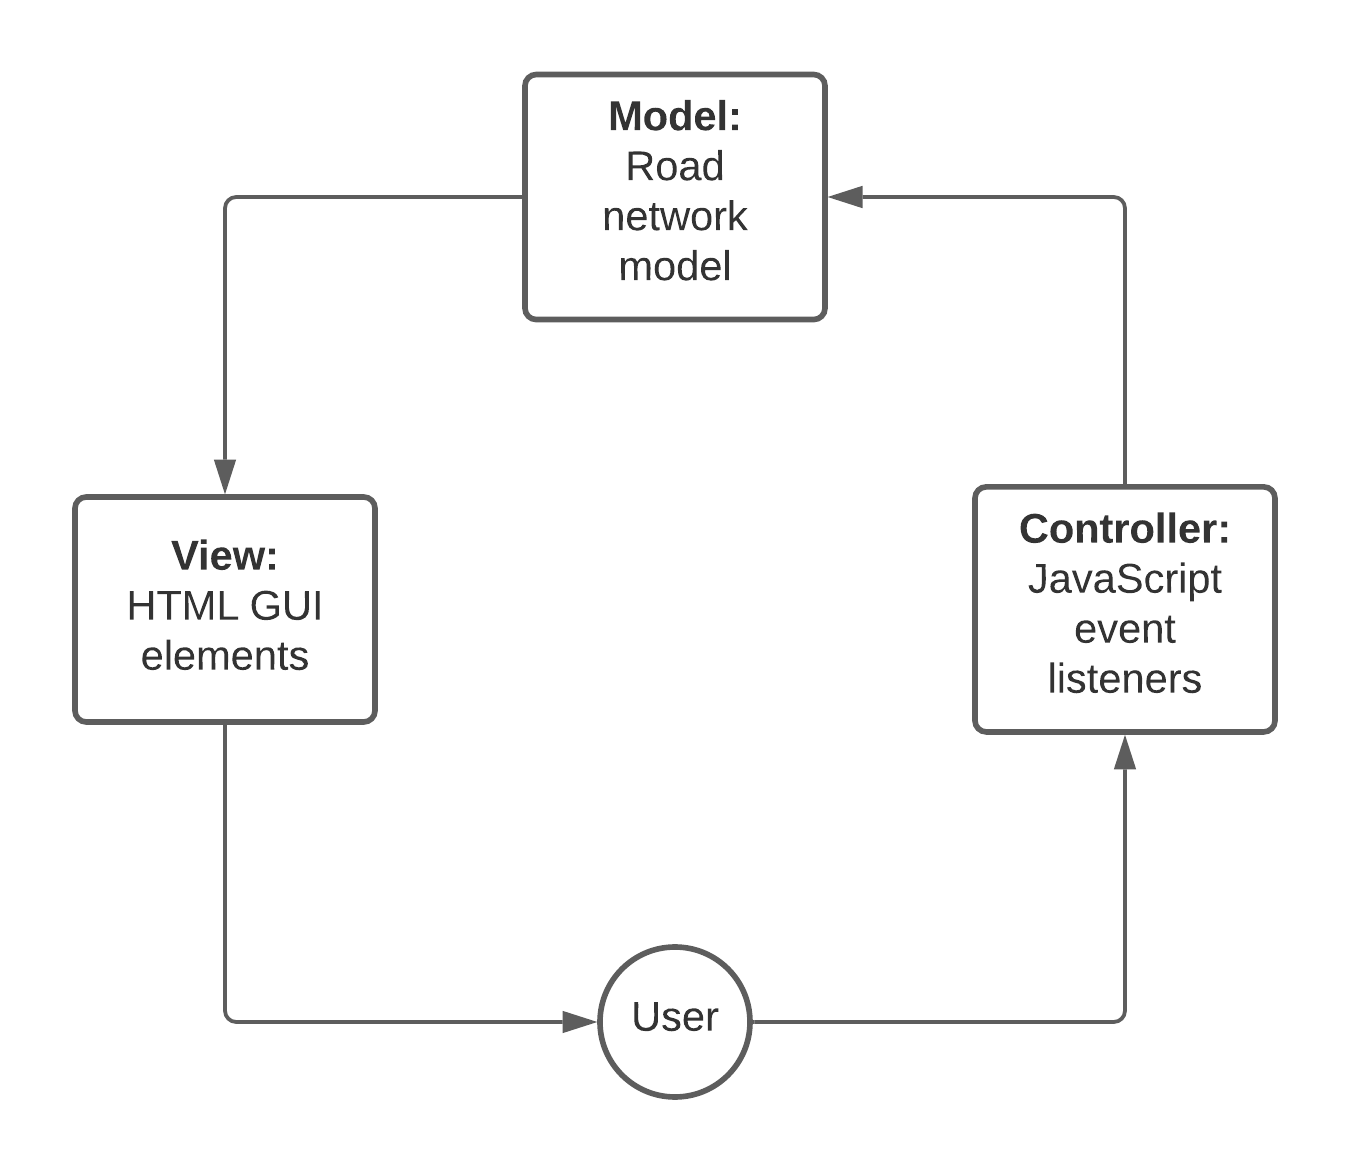
\includegraphics[width=0.5\textwidth]{model-view-controller.png}
        \caption{Model-view-controller design pattern}
        \label{model-view-controller}
    \end{figure}

    Note that in this framework the 'Model' includes both the Road network model and the testing component together, although these will be separately implemented.

\section{Network Builder}

    \subsection{User Interaction}

    As specified in my analysis section, the user input scheme will be based largely off of mouse interactions similar to that of the Mini Motorways computer game [\autoref{mini-motorways}]. The controls are listed in \autoref{user-interaction-specification}:

    \begin{table}[ht]
        \centering
        \begin{tabular}{|p{0.45\textwidth}|p{0.45\textwidth}|}
            \hline
            \textbf{Input} & \textbf{Result}\\
            \hline
            Left-click on existing node and drag to another existing node & Connect a road between the two targeted vertices\\\hline
            Left-click on existing node and drag to empty space & Create new node at the end point and connect with the existing node\\\hline
            Shift-Left-click on empty space & Create new node at the selected point with no connections\\\hline
            Shift-Left-click on existing node and drag & Move the targeted node along the path of the cursor until button is released\\\hline
        \end{tabular}
        \caption{User interactions with graph model}
        \label{user-interaction-specification}
    \end{table}

    This program will include undo/redo functionality on the network construction component specifically, this will be modelled using two stacks, one containing the user actions that have occurred (the previous states stack) and the other containing the actions that have been reapplied from the previous states stack (the future states stack). \autoref{undo-redo-diagram} shows a diagram of the undo-redo procedures, popping from one stack and pushing into the other.

    \begin{figure}
        \centering
        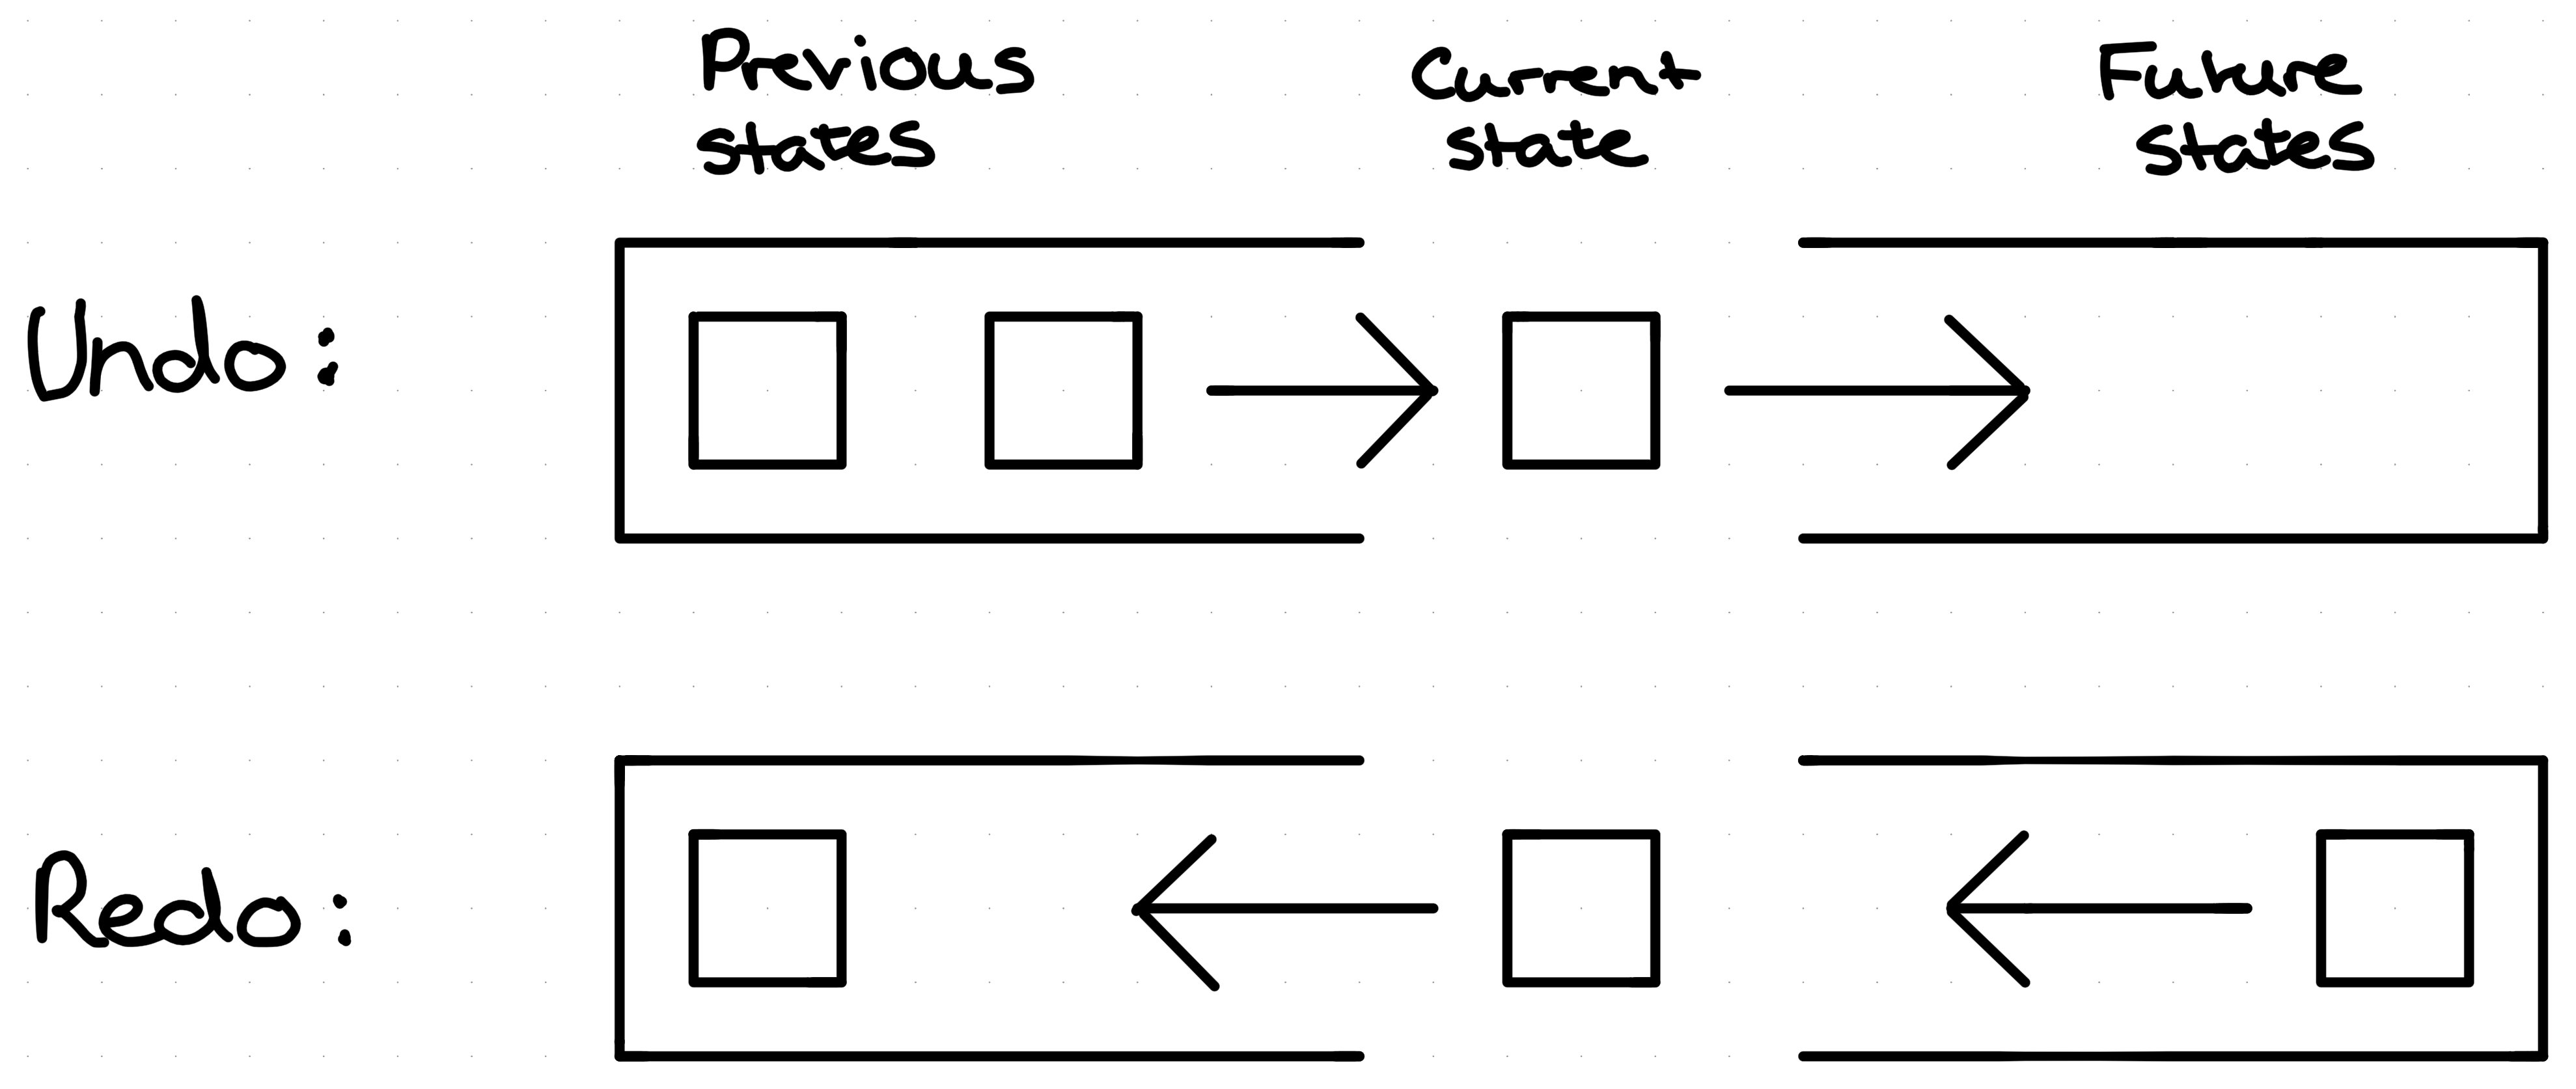
\includegraphics[width=0.9\textwidth]{undo-redo-diagram.jpg}
        \caption{Diagram showing the undo-redo procedures}
        \label{undo-redo-diagram}
    \end{figure}

    \subsection{Graph Structure}

        After exploring the different types of graph structure I have decided to utilise the adjacency matrix structure for this project. Despite the adjacency matrix implementation having less scalable complexities for most functions [\autoref{graph-time-complexities}] it has a large benefit of a constant time edge lookup; since this function will be called many times for each agent in the network I anticipate this implementation will be more efficient in the long term. The necessary fuctions that need to be included in this graph implementation are listed in \autoref{graph-functions}

        \begin{table}[ht]
            \centering
            \begin{tabular}{|p{0.45\textwidth}|p{0.45\textwidth}|}
                \hline
                \textbf{Method definition} & \textbf{Description}\\
                \hline
                \inlinecode{add_vertex(vertex): integer} & Adds a new vertex to the graph with a specified vertex value, returning the index of the new vertex\\
                \hline
                \inlinecode{set_vertex(vertexId, value): void} & Sets the value of a vertex at a given vertex id, no return value\\
                \hline
                \inlinecode{get_vertex(vertexId): Vertex} & Returns the value of a vertex at a given vertex id\\
                \hline
                \inlinecode{remove_vertex(vertexId): Vertex} & Removes a vertex from the graph at a given vertex id, returning the value of the removed vertex\\
                \hline
                \inlinecode{set_edge(srcId, dstId, value): void} & Sets the value of the edge starting from the vertex at the source id and ending at the vertex at destination id\\
                \hline
                \inlinecode{get_edge(srcId, dstId): Edge} & Returns the value of an edge between the source vertex and destination vertex\\
                \hline
                \inlinecode{remove_edge(srcId, dstId): Edge} & Removes the edge between the source and destination vertices, returning the value of the edge\\
                \hline
            \end{tabular}
            \caption{Specification for the graph class implementation}
            \label{graph-functions}
        \end{table}

    \subsection{Road geometry}

    The roads will be moddeled using a series of Bezier curves, to allow for this the user must be able to adjust the control points of the curves. The edges of the graph will need to store a data structure containing 2 control points for the curve (the first and last points are defined by the source and destination nodes of the edge). This will make for cubic Bezier curves which will be controlled by their own \inlinecode{CubicBezier} class. One function of this will be a \inlinecode{get_point} method which will interpolate linearly along the length of the curve, return a point. This is not a trivial problem and my solution is documented below.

    \paragraph{Linear interpolation of cubic Bezier curves}

    Given a cubic Bezier curve with control points $\mathbf{P_0}$, $\mathbf{P_1}$, $\mathbf{P_2}$ and $\mathbf{P_3}$. We can define it as

    \[B(t) = (1 - t)^3\mathbf{P_0} + 3(1 - t)^2t\mathbf{P_1} + 3(1 - t)t^2\mathbf{P_2} + t^3\mathbf{P_3} : 0 \leq t \leq 1\]

    As shown in \autoref{non-linear-interpolated-bezier}, the $t$ parameter does not interpolate linearly across the curve. The distances between successive points is not constant. This is an issue as cars will need to move at a given speed along these curves.

    \begin{figure}
        \centering
        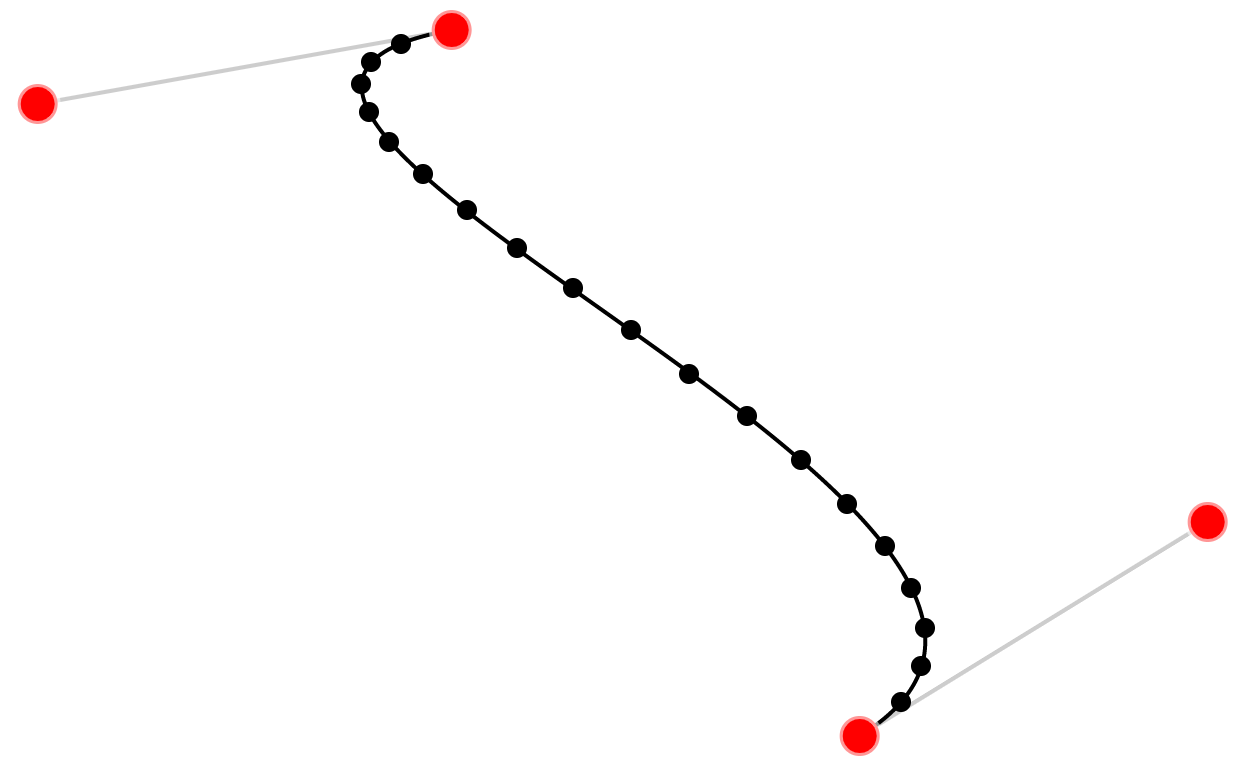
\includegraphics[width=0.4\textwidth]{non-linear-interpolated-bezier.png}
        \caption{Bezier curve with equally spaced points by $t$-value}
        \label{non-linear-interpolated-bezier}
    \end{figure}

    In order to achieve this I will need to compute the arc length of the Bezier curve. Allowing me to take steps with respect to distance instead of $t$-value.

    The arc length can be represented by summing many small steps along the curve, the distance along the curve to some $t = z$ can be represented in integral notation as:

    \[\int_0^z\sqrt{\left(\frac{dx}{dt}\right)^2 + \left(\frac{dy}{dt}\right)^2}dt\]

    It can be shown that a closed form solution does not exist \cite{no-closed-form-bezier} for Bezier curves of order greater than 2. So we must use an approximate method to compute these values. However square roots are very expensive computationally, so it would be inefficient to compute this many times for every call. My solution to this is to build a graph that maps distances to $t$-values using a sequence of samples, \autoref{t-against-distance}
    \begin{algorithm}
        \begin{algorithmic}
            \Function{get\_arc\_length}{B, z}
                \State distance $\gets 0$
                \State $t \gets 0$
                \While{$t < z$}
                    \State $p \gets$ \Call{B.get\_point}{t}
                    \State $t \gets t + 0.01$
                    \State $q \gets$ \Call{B.get\_point}{t}

                    \State distance $\gets$ distance $+ \sqrt{(p_x - q_x)^2 + (p_y - q_y)^2}$
                \EndWhile
                \State \textbf{return} distance
            \EndFunction
        \end{algorithmic}
        \caption{Computing the arc length along a Bezier curve}
        \label{numerical-integration}
    \end{algorithm}

    \subsection{GUI}

\section{Network Testing}

    \subsection{Traffic Behaviour Modelling}

    \subsection{Agent Structure}

    \subsection{Maximum Graph Flow}

    \subsection{GUI}

    \subsection{Bezier Curvature}
